\section{Set definitions for the RMPC}

For the RMPC algorithm, we need to define some of the sets which were used in the RMPC formulation.

\subsection{Approximating the bounding sets for the input}
\label{sec:approx input sets}
Given $x \in X$, define the set $V(x) \defeq \{v \in \Re^{\dimV} \such u(x) = R^{-1}(x)[b(x)+v] \in U\}$.
We assume that there exist functions $\ua{v}_i, \oa{v}_i: X \rightarrow \Re$ s.t. for any $x$, $V(x) = \{[v_1,\ldots,v_{\dimV}]^T \such \ua{v}_i(x) \leq v_i \leq \oa{v_i}(x) \}$.
Because in general $V(x)$ is not a rectangle, we work with inner and outer rectangular approximations of $V(x)$.
Specifically, let $\Xc$ be a subset of $X$.
Define the inner and outer bounding rectangles, respectively
\[\ua{V}(\Xc) \defeq \{v=[v_1,\ldots,v_{\dimV}]^T \such \max_{x\in \Xc} \ua{v}_i(x)  \leq v_i \leq \min_{x \in \Xc} \oa{v}_i(x) \} \]
\[\oa{V}(\Xc) \defeq \{v=[v_1,\ldots,v_{\dimV}]^T \such \min_{x\in \Xc} \ua{v}_i(x)  \leq v_i \leq \max_{x \in \Xc} \oa{v}_i(x) \} \]

By construction, we have for any subset $\Xc \subset X$
\begin{equation}
\label{eq:Vbounds}
\ua{V}(\Xc) \leq \cup_{x \in \Xc} V(x) \subset \oa{V}(\Xc)
\end{equation}
If two subsets of $X$ satisfy $\Xc_1 \subset \Xc_2$, then it holds that 
\begin{eqnarray}
\label{eq:V inclusions}
\ua{V}(\Xc_2) \subset \ua{V}(\Xc_1)
\nonumber
\\
\oa{V}(\Xc_1) \subset \oa{V}(\Xc_2)
\end{eqnarray}


\subsection{Approximating the bounding sets for the disturbances}
\label{sec:approx dist}
We will also need to define containing sets for the state estimation error in $z$ space:
Recall, we have $\hat{z}_k = T(\hat{x}_k) = T(x_k+e_k)$. We assume that the magnitude of $e_k$ is small w.r.t the magnitude of $x_k$. With this, we do a Jacobian Linearization as follows

\begin{subequations}
\label{eq:err_lin}
\begin{align}
&\hat{z}_k = T(x_k) + \frac{d}{dx_k} T(x_k+e_k)|_{e_k=0}e_k + O(e^2) \\
&\text{Ignoring the higher order terms} \nonumber \\
&\approxeq z_k + M(x_k)e_k  \\
&\text{And therefore} \nonumber \\
&\tilde{e}_k = \hat{z}_k - z_k = M(x_k)e_k
\end{align}
\end{subequations}

This gives us an additional representation of the estimation error in $z$ in terms of the current state $x_k$ and $e_k$, where $M(x_k)$ is the appropriately sized Jacobian matrix. 

So for any $k,j$, $\hat{z}_{k+j} = T(\hat{x}_{k+j}) = T(x_{k+j} + e_{k+j}) \approxeq T(x_{k+j}) + M(x_{k+j})e_{k+j} = z_{k+j} + M(x_{k+j})e_{k+j} = z_{k+j} + \te_{{k+j}}$.
Therefore the state estimation error $\te_{k+j}$ lives in 
$\cup_{x\in X_{k+j|k}, e \in E}M(x)e = \cup_{x \in X_{k+j|k}}M(x)E$, 
where $X_{k+j|k}$ is the $j$-step reach set of the nonlinear dynamics computed starting at time $k$ and given $\hat{x}_k$, since we only have access to the estimate and not the true state.

It is reasonable to assume that the linearization of Eq. \ref{eq:err_lin} allows us to compute accurate bounds on $\te_{k+j}$ when the estimation error is small. For the running example of Eq. \ref{eq:toy_dynamics}, we have $M = [1 \, 0;0 \,a\cos(x_2)]$. Starting with an estimation error bound on $e_k$ of the form (in radians) $E = \lbrace e| ||e||_{\infty} \leq 0.0227\rbrace$, i.e. the absolute value of estimation error in $x_1$ is $1.3\degree$ and for $x_2$ is bounded by $1.3\degree s^{-1}$, and the safety bound $|x_2|\leq 0.8660$ as computed in Sec. \ref{sec:formulation}, Fig. \ref{fig:fb_err} shows the expected error in linearization for the estimation error term $\tilde{e}_2$ as a function of $x_2$ (it is only a function of $x_2$). It shows that over the entire range of $x_2$, this error is very small even when normalized by $T(\hat{x_2})$. Note $\tilde{e}_1 = e_1$ (see $M$ above), therefore there is no linearization error in that term.


\begin{figure}
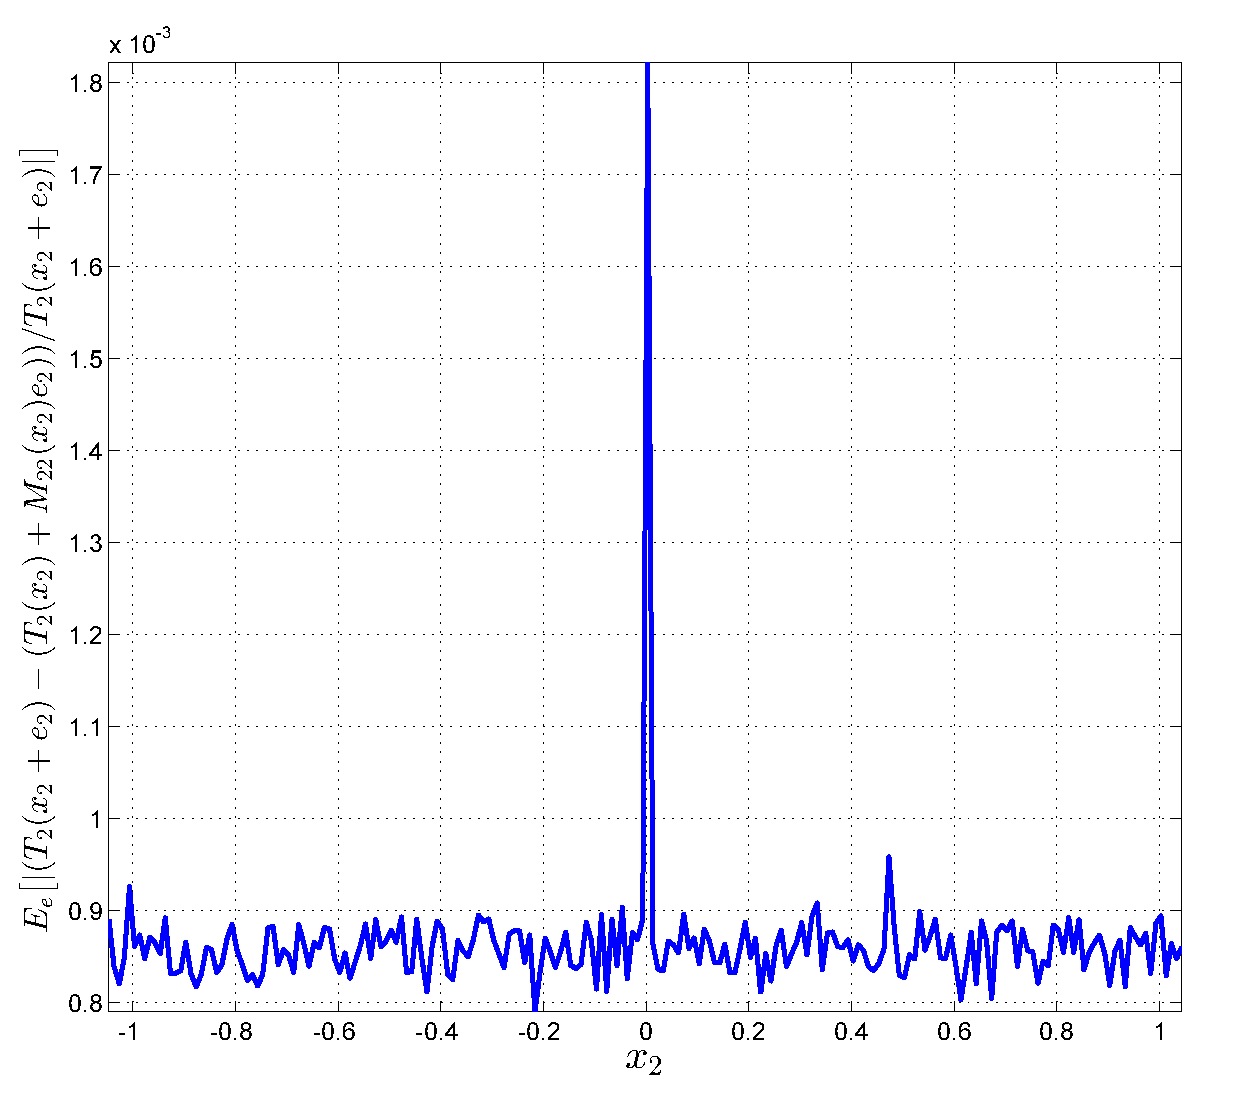
\includegraphics[width=0.49\textwidth]{figs/Toy_LinErrEst_scissored.pdf}
\caption{Expected linearization error in $\tilde{e}_2$ as a function of $x_2$ for the running example. Note, the peak at $x_2=0$ is expected due to the form of $T(x)$. }
\label{fig:fb_err}
\end{figure}
